% !TEX root = SystemTemplate.tex

\chapter{System  and Unit Testing}

This section describes the approach taken with regard to system and unit testing. 

\section{Overview}
Provides a brief overview of the testing approach, testing frameworks, and general 
how testing is/will be done to provide a measure of success for the system. 



\section{Dependencies}
Describe the basic dependencies which should include unit testing frameworks and 
reference material. 


\section{Test Setup and Execution}
Describe how test cases were developed, setup, and executed.  This section can 
be extremely involved if a complete list of test cases was warranted for the system. 


\begin{table}[tbh]
\caption{The texting Matrix For CrowdControl. \label{testingmatrix}}
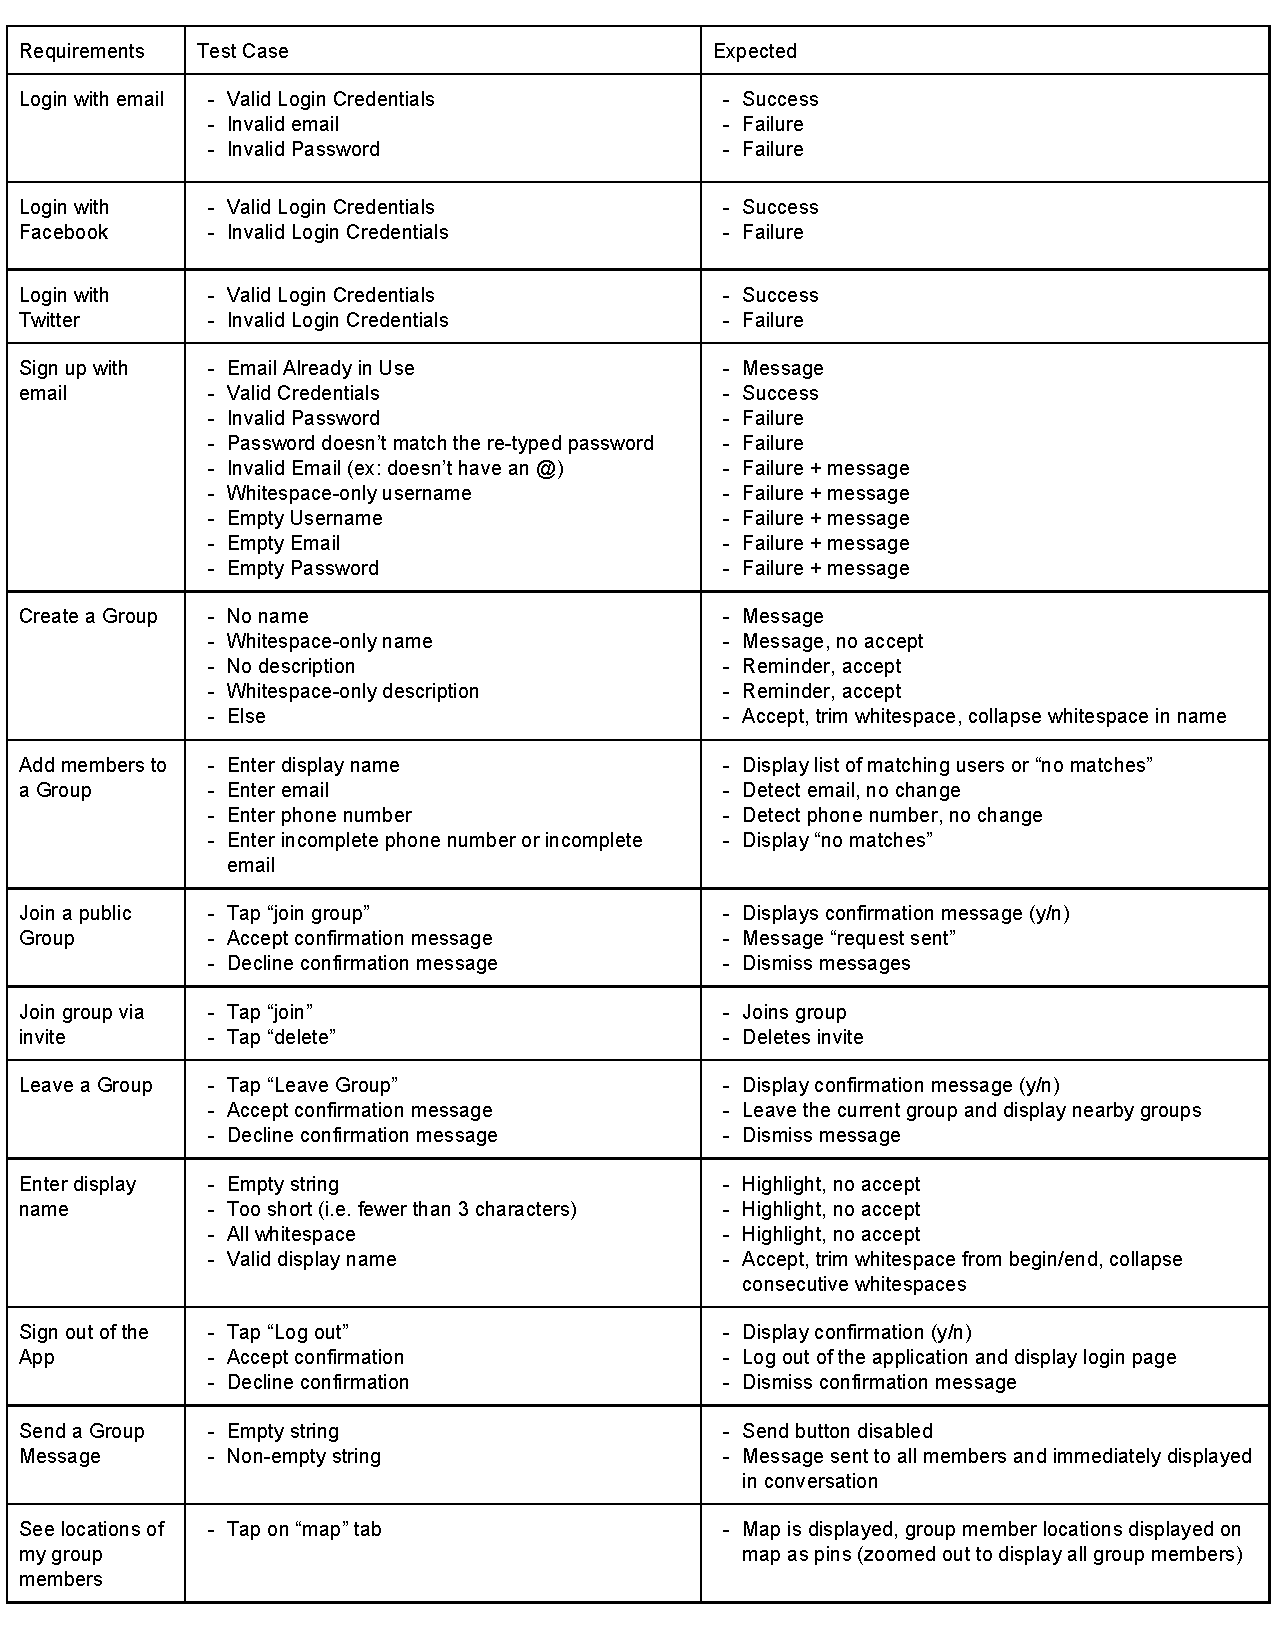
\includepdf{DesignPictures/TestingMatrix.pdf}
\end{table}

